\documentclass{report}
\usepackage[utf8]{inputenc}
\usepackage[right=30mm,left=30mm]{geometry}
\usepackage{microtype}
\usepackage[T1]{fontenc}
\usepackage{natbib}
\usepackage[francais]{babel}
\usepackage{fourier}
\usepackage{amssymb}
\usepackage{mathrsfs}
\usepackage{xspace}
\usepackage{lmodern}
\usepackage{amsmath}
\usepackage{graphicx}
\usepackage{hyperref}
\usepackage{lscape} %% mettre une page au format portrait (landscape)
\usepackage{xcolor}
\hypersetup{
	colorlinks=true,
	breaklinks=false,
	urlcolor= blue,
	linkcolor= blue,
	citecolor= blue}
\frenchbsetup{
	CompactItemize=false,         % ne pas compacter les listes
	%ThinSpaceInFrenchNumbers=true % espace fine dans les nombres
}
\usepackage[mediumspace,mediumqspace,squaren]{SIunits} %utilisé pour les unités (micromètre)
%\usepackage[options]{natbib}: citation en chifres dans le texte.

\newcommand{\Ctreize}{$\delta$\textsuperscript{13}C\xspace}

\newcommand{\Odixhuit}{$\delta$\textsuperscript{18}O\xspace}

\title{Proposé de recherche}
\author{André Soro}
	
\begin{document}
	
	\maketitle
	\tableofcontents
	\listoffigures
	


%\part*{Introduction et problématique}
\chapter*{Introduction et problématiques}
\phantomsection\addcontentsline{toc}{chapter}{Introduction} % inclure dans TdM

L'épinette blanche (\textit{Picea glauca} (Moench) Voss) est une espèce d'arbre qui a une grande importance dans les forêts du Québec et plus largement du Canada. Elle a une valeur économique importante du fait de sa distribution géographique et de son abondance (Figure~\ref{fig:distribution}). Le bois d'épinette est apprécié comme bois de construction, comme matériel pour des produits de menuiserie et pour la mise en pâte grâce aux caractéristiques de ses fibres \citep{Zhang2008}. Ainsi, l'épinette blanche est fortement reboisée dans  divers systèmes sylvicoles au Canada \citep{Canadian2009}. Cette espèce présente une certaine plasticité, car elle est capable de s'adapter à divers types de sols et conditions climatiques \citep{Nienstaedt1990}. Les propriétés physiques du bois d'épinette sont principalement liées à son anatomie \citep{Rossi2012} etc. Les variations de certains caractères anatomiques du bois tels que la largeur des cernes et de certaines propriétés, notamment la densité du bois, dépendent de l'activité cambiale (activité du cambium), qui elle est régie par deux conditions principales: génétiques et environnementales \citep{Dufour2010,Rossi2012}. La densité est influencée par le diamètre cellulaire et l'épaisseur de la paroi. Elle est donc un caractère indirect influencé par des caractères anatomiques. L'activité cambiale va strictement influencer le nombre de cellules formées (largeur de cerne) et d'autres facteurs comme la durée de vie des initiales va déterminer entre autre combien de matériel (épaisseur) peut être déposé lors de la maturation cellulaire. Depuis les années 1950, plusieurs études se sont intéressées à la variation génétique et phénotypique influençant la croissance des arbres et les caractéristiques du bois \citep{Corriveau1971,Li1993,Li1997}. Initialement, les programmes d'améliorations génétiques s'intéressaient principalement à la croissance rapide des arbres et visaient ainsi à augmenter la croissance en volume des plantations futures. En revanche, les  propriétés mécaniques et l'anatomie du bois étaient peu considérées dans ces programmes de façon générale \citep{Zhang1995}. Certaines recherches se sont intéressées à évaluer les variations génétiques des propriétés (mécaniques) du bois, telles que la densité du bois, la longueur des fibres et leur impact sur la production du bois \citep{Hernandez2001,Beaulieu2003}. De plus en plus d'études se penchent sur la génétique des propriétés radiales du bois telles que la densité, la rigidité du bois, la résistance à la flexion et l'angle des microfibrilles \citep{Lenz2010,McLean2016} pour obtenir une meilleure compréhension du contrôle génétique de ces caractères et les possibilités d'inclure la qualité du bois comme critère de sélection dans les programmes d'amélioration génétique de l'épinette blanche. \cite{Lenz2011} ont étudié les relations entre les propriétés du bois notamment la densité du bois, l'angle des microfibrilles (AMF) et le module d'élasticité ainsi que la croissance radiale chez \textit{Picea glauca}. Les auteurs ont trouvé que le niveau de corrélation est variable avec l'âge cambial et change du bois juvénile au bois mature. Leurs travaux ont montré une absence de corrélations entre l'AMF et la densité du bois; entre l'AMF et les propriétés liées à l'anatomie des fibres telles que le diamètre des fibres et l'épaisseur de la paroi. \\ 

\begin{figure}
	
	\centering
	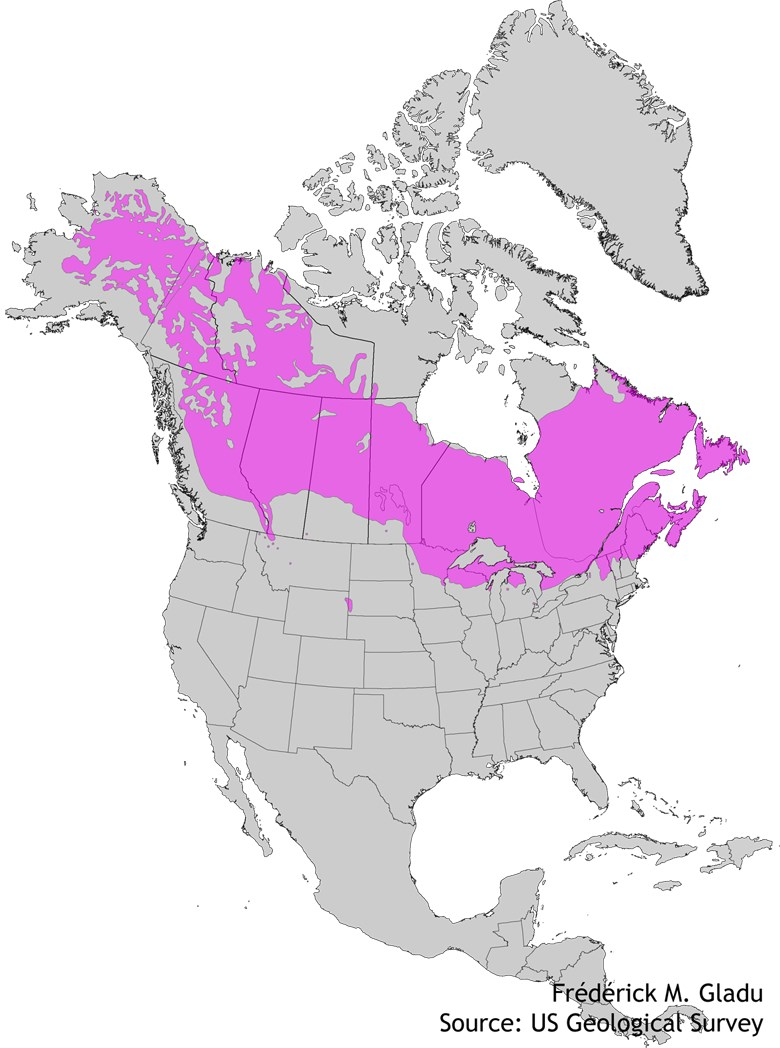
\includegraphics[width=0.65\textwidth]{distribution.jpg}
	\caption{Distribution de l'épinette blanche au Canada}
	\label{fig:distribution}
	
	
\end{figure}


\cite{Ivkovich2002} ont trouvé une relation entre différents caractères anatomiques du bois d'épinette, notamment l'angle des microfibrilles, et la densité à l'aide de carottes prélevées à hauteur de poitrine (DHP).Dans leur étude, ils ont observés que l'analyse des composantes anatomiques n'apporte pas un avantage précis pour éviter la relation négative qui existe entre la croissance et la densité du bois. D'autres études sur la densité du bois ont mis en évidence un lien entre la densité du bois et rigidité en flexion, et la résistance mécanique du bois scié \citep{Saranpaa1994,Alteyrac2006}. Ces résultats soulignent le caractère clé de la densité parce qu'elle est l'un des indicateurs de la qualité du bois les plus largement utilisés. Ainsi, elle affecte la performance du bois scié, l'aptitude à la fabrication de panneaux et les rendements en pâte \citep{Macdonald2002}. La densité du bois influence aussi le calcul des valeurs calorifiques pour les applications de biomasse pour la bioénergie \citep{Mckendry2002}. Elle peut être variable au sein d'une même espèce en lien avec les conditions environnementales ou d'une même famille. Par conséquent, Les modèles de prédiction de la densité du bois prennent en compte l'âge cambial \citep{David2014}, la génétique et les conditions météorologiques \citep{Wilkinson2015}. L'importance de la densité pour la qualité du bois est la raison pour laquelle nous nous intéresserons à e caractère dans notre étude. \\

Au Québec, les prochaines sélections génétiques dans les programmes d'amélioration des différentes espèces d'épinettes considéreront l'héritabilité des propriétés du bois \citep{Mullin2011, Beaulieu2009}. Par définition, l'héritabilité est une donnée statistique qui sert à évaluer la part des facteurs génétiques et celle des facteurs environnementaux dans la construction du phénotype d'une population donnée. \cite{Lenz2010} ont étudié l'héritabilité des caractéristiques d'anatomie cellulaire du bois d'épinette blanche en fonction de l'âge cambial. Leur étude a montré que la part du facteur génétique pour les caractéristiques d'anatomie cellulaire augmente avec l'âge cambial. Par contre, le contrôle génétique de l'AMF est constant.  En outre, \cite{Lenz2011} ont étudié les relations génétiques entre caractères du bois et leurs conséquences sur l'amélioration des arbres. Ces études ont montré que les propriétés du bois pourraient être contrôlées en partie par la génétique. Toutefois, l'amélioration génétique à elle seule n'est pas suffisante pour assurer une amélioration des propriétés du bois. Des facteurs tels que les conditions environnementales semblent influencer les propriétés du bois et leurs effets peuvent varier en fonction du bagage génétique des arbres. De ce fait, l'amélioration des propriétés du bois doit prendre en compte à la fois l'amélioration génétique et les conditions climatiques. \\

Le climat est un facteur déterminant pour la croissance et les processus physiologiques des arbres. Ainsi, les conditions climatiques affectent fortement les propriétés du bois. En effet, certains facteurs climatiques comme la sécheresse peuvent engendrer un stress chez les arbres et entraîner une variation des propriétés du bois, notamment la densité et largeur des cernes. La disponibilité en eau qui est dépendante du climat, est un facteur important qui influence la croissance des arbres \citep{Lebourgeois2005} et un déficit hydrique est une source de stress qui affecte les processus physiologiques \citep{Waring1987}. Par conséquent, il est important de déterminer les potentiels effets des changements climatiques sur la qualité du bois et son héritabilité dans une optique de reboisement. En effet, les modèles de climat futur prévoient des changements de régime hydrique avec des périodes plus importantes de dessiccation et de désaturation des sols \citep{IPCC_2015}. Cela explique l'intérêt de plusieurs études sur l'impact potentiel des variations climatiques sur la qualité du bois. \\

Plusieurs études antérieures se sont intéressées à l'effet des conditions environnementales sur les propriétés du bois. L'environnement (climat, disponibilité en eau, etc.) affecte directement l'activité cambiale de l'arbre \citep{FRITTS1976,Kozlowski1997}. La division des cellules cambiales étant responsable de la quantité et de la qualité du bois \citep{Begum2013}, les conditions environnementales peuvent donc influencer la qualité du bois. L'impact météorologique sur la qualité du bois varie d'un site à l'autre en fonction des types de stress auxquels sont exposés les arbres. Dans les régions où les arbres sont très exposés au vent, par exemple, ils auront tendance à former du bois de réaction. Les précipitations peuvent aussi affecter la qualité du bois dans certaines régions. \cite{Bouriaud2005} ont trouvé une forte corrélation positive entre le déficit en eau du sol et la densité du bois. Un déficit d'eau dans le sol peut ralentir la croissance, ce qui peut entraîner une augmentation de la densité du bois \citep{GARDINER2011}. En plus, l'impact climatique sur l'anatomie du bois a été montré dans plusieurs études \citep{Bouriaud2005,Fritts2001,Campelo2013}. Ces études montrent un effet du climat sur la croissance des arbres, sur la variation intra-annuelle de la densité. Dans certaines études, la variation des propriétés du bois telles que la largeur de la paroi cellulaire \citep{Fritts2001}, la croissance radiale \citep{Jyske2009}, la variabilité intra-annuelle de la densité du bois \citep{Wimmer2000,Rigling2001,Wilkinson2015} a été utilisée comme marqueur de sécheresse. Ces études ont mis en évidence que les fluctuations climatiques peuvent conduire à des variations intra-annuelles de la densité du bois. \\

La densité du bois peut avoir des variations inter et/ou intra-annuelles au sein d'un même arbre. \cite{Fritts2001}, définit les variations intra-annuelles de la densité du bois comme la présence de cellules semblables au bois initial dans le bois final et/ou la présence de cellules semblables au bois final dans le bois initial. Ces variations intra-annuelles de la densité sont induites par une variation des conditions environnementales durant la période de croissance radiale. L'activité cambiale est donc modifiée, ce qui peut fournir des informations sur les conditions climatiques \citep{Campeloa2007,Campelo2013,Novak2013}. Par conséquent, l'étude de la variation de la densité intra-annuelle permet d'avoir des informations sur l'environnement et inversement. Les variations inter-annuelles, par contre, peuvent être induites par les conditions environnementales lors de la période de croissance, de l'année précédente ou par l'activité écophysiologique annuelle \citep{Hughes1984,DArrigo1992}. Elles se définissent par une variation de la densité et/ou de la largeur des cernes d'une année à l'autre. La compréhension de la variation de la densité est alors nécessaire dans une optique d'anticipation de l'impact du climat futur sur la qualité du bois. Parmi les méthodes utilisées pour la compréhension de l'effet du climat sur les propriétés du bois nous avons l'utilisation des isotopes qui prend de plus en plus d'ampleur. Les isotopes sont des nucléides qui ont le même nombre de protons, mais ayant un nombre de neutrons différent.\\

De plus en plus d'études récentes utilisent l'analyse isotopique qui est une analyse de la structure fine (isotopes stables) du bois formé lors des événements climatiques particuliers pour faire le lien entre la variabilité des propriétés du bois telles que la largeur du cerne, la densité du bois et les conditions climatiques. La plupart des éléments chimiques contiennent plus d'un isotope stable, qui se définit comme un isotope qui ne subit pas de désintégration radioactive dans le temps \citep{West2006}. La plupart des processus biochimiques et biogéochimiques sont associé à un filtre isotopique en défaveur des isotopes lourds dans les mélanges chimiques (p.ex. \up{18}O plus que \up{16}O). Ce filtre isotopique entraîne une variation isotopique des pools de sources et de produits à différentes étapes d'un cycle biogéochimique et des ressources utilisées par les organismes de ces pools \citep{Dawson2002}. Le passage du carbone de l'atmosphère aux feuilles de la plante par la photosynthèse est un processus qui discrimine contre le \up{13}C. L'ouverture et la fermeture des stomates de la plante influencent cette discrimination. En effet, la fermeture des stomates entraîne une modification de la signature isotopique du carbone et de l'oxygène dans le bois \citep{Farquhar1993, Bigras2005}.
L'air interne des feuilles est appauvri en \up{13}C par rapport à l'air ambiant, ce qui entraîne un «fractionnement dû à la diffusion». Si l'ouverture stomatique est extrêmement petite (0,1 mm), les collisions avec les cellules de garde deviennent importantes et le fractionnement est beaucoup plus élevé, mais cela ne se produit que chez les espèces avec une fréquence élevée de très petits stomates tels que les Citrus (\textit{Citrus glauca} et Microcitrus) \citep{Farquhar1993}. Une fermeture des stomates suite à un déficit d'eau peut avoir le même effet. Par conséquent, la composition des isotopes stables du carbone et de l'oxygène du bois est de plus en plus intégrée dans les travaux qui ont pour but de déduire les conditions climatiques et les réactions physiologiques des arbres \citep{McCarroll2004, Sternberg2009,Sarris2013}. \\

Les méthodes basées sur la mesure d'isotopes stables sont parmi les outils les plus précis pour la compréhension des relations entre les plantes et leur environnement \citep{Dawson2002}. Les isotopes sont inégalement répartis entre et au sein de différents composés, et cette distribution isotopique peut mettre en évidence des informations sur différents processus, notamment physiques, chimiques et métaboliques impliqués dans les transformations du carbone \citep{Farquhar1989}. L'utilisation des méthodes basées sur les isotopes de carbone stables dans le matériel végétal, et particulièrement dans les cernes annuels, s'est généralisée quand le modèle de \cite{Farquhar1989} est devenu un modèle prédictif des effets environnementaux sur les rapports isotopiques. La proportion d'isotopes stables (\Ctreize et le \Odixhuit) dans une partie de la plante varie suite aux processus physiques et biologiques. Le fractionnement isotopique ($\Delta$) est la discrimination de l'isotope lourd en faveur de l'isotope léger. La composition en isotopes stables du bois et de la cellulose peut être utilisée pour expliquer certains mécanismes dendroclimatiques. La cellulose est le constituant principal du bois et donc le plus utilisé pour les mesures de \Odixhuit et \Ctreize dans les arbres. Le \Ctreize et le \Odixhuit du bois et les constituants du bois dans les cernes annuels peuvent refléter les conditions météorologiques subies par l'arbre \citep{Duquesnay1998,McCarroll2004,Hartl-meier2015}. Des méta-analyses ont montré une corrélation entre la variation isotopique de la biomasse de la plante et les précipitations moyennes. Le fractionnement isotopique du carbone et de l'oxygène pendant la photosynthèse est également utile pour évaluer l'impact environnemental sur les variations intra-annuelles de la densité \citep{Farquhar1989,JonLloyd1994}. Les isotopes du carbone et de l'azote sont aussi utilisés pour caractériser la variation intra-annuelle de la densité. Des études récentes ont montré que l'anatomie du bois couplée aux isotopes stables (\Ctreize et \Odixhuit) permettent une meilleure interprétation entre variations intra et interannuelles de densité et la physiologie de l'arbre \citep{Micco2007,Vaganov2009,Sarris2013}. Le \Odixhuit dans le bois est relié à la quantité de précipitations \citep{Bonal2000} et il existe une relation entre le \Ctreize et la fermeture des stomates qui elle est relié à la température et aux précipitations \citep{Pons2011}. Par conséquent, l'utilisation couplée du \Ctreize et du \Odixhuit permet une prise en compte à la fois des précipitations et de la température de l'air (conditions climatiques plus précises) dans la compréhension de la relation entre conditions climatiques et signature isotopique des anneaux annuelles de croissance. \\ % AA il me semble que tu restes un peu en surface. Pour la présentation orale, j'aimerais que tu utilises des graphiques et que tu prennes une optique plus pédagogique. On en reparlera de vive-voix.

La réaction de l'arbre face à certains stress climatiques notamment la sécheresse peut être fonction de l'intensité de celle-ci. Afin, de prendre en compte les potentielles conséquences des changements climatiques qui selon les prévisions vont occasionner des sécheresses de plus en plus intenses et fréquentes \citep{IPCC_2015}, il est important d'inclure des données récoltées dans des conditions de sécheresse intense dans nos modèles pour une meilleure prédiction.\\
Les expériences avec stress climatique intense et les modèles qui prennent en compte ces effets permettront de faire des améliorations génétiques pour des résultats qui aboutissent à une production de bois de bonne qualité.\\

De façon générale, les travaux qui ont montré une relation entre la sécheresse et les propriétés du bois ont été réalisés sur des arbres qui n'ont pas subi un stress constant/intense ou étaient en irrigation \citep{Xu2012,Drew2009,Campelo2013,Jyske2009,Wilkinson2015}. En revanche, l'effet potentiel qu'une sécheresse intense peut avoir sur la densité du bois est peu connu.\\ %AA: L'article de Wilkinson touche directement à ça. Il faudrait aller un peu plus loin en expliquant ce qu'ils ont trouvé

Le bilan de la littérature met en évidence que l'effet des conditions météorologiques et le contrôle génétique des propriétés du bois ont été souvent étudiés séparément. Des études récentes ont trouvé une relation entre les conditions climatiques comme la sécheresse, la température et du contrôle génétique sur les propriétés du bois \citep{Housset2018, Heer2018}. Ils ont observé un lien direct entre les caractères dendroécologiques et la génétique. Ces études font un lien entre la résilience des arbres aux variations climatiques et le contrôle génétique, par contre l'héritabilité de ces caractères de résilience est très peu connue. Notre étude permettra de mieux connaître l'héritabilité de la réaction des arbres face aux variations climatiques notamment à la sécheresse. Les résultats pourront être utilisés pour l'amélioration génétique et permettre d'anticiper les effets des changements climatiques sur la production et la qualité du bois. \\

%AA: J'ai réalisé en lisant les commentaires de patrick sur le texte d'Iman que l'héritabilité peut se définir de deux manières. Quelque part dans ton texte, tu dois donner ces explications. Voir le proposé de Patrick


\section*{Objectifs}
\phantomsection\addcontentsline{toc}{section}{Objectifs}

Ce projet a pour objectif de lier la variation des propriétés du bois au climat et d'évaluer le contrôle génétique de cette variation des propriétés aux conditions environnementales dans des populations d'épinettes blanches utilisées dans le programme d'amélioration génétique au Québec. Parmi les conditions environnementales, l'étude se focalisera notamment sur les effets des précipitations et des stress hydriques, alors que les propriétés du bois évaluées seront notamment la largeur des cernes, la densité du bois, l'angle moyen des microfibrilles de cellulose dans la paroi cellulaire et la proportion en isotopes stables de \Ctreize et \Odixhuit. Le projet sera élaboré en trois chapitres qui permettront la rédaction d'autant d'articles scientifiques. Les objectifs spécifiques de chacun des chapitres sont les suivants:\\

\begin{itemize} 
	
	\item Caractériser les profils de densité et de largeur des cernes afin d'identifier les familles ayant produit le bois le plus « uniforme » au cours des années, et ce, malgré les possibles variations environnementales. 
	
	\item Évaluer l'influence de différents niveaux de stress hydrique imposé artificiellement sur les propriétés du bois de jeunes semis; ensuite mesurer la variabilité de la réaction au stress parmi différents croisements et clones. 	
	
	\item Déterminer les impacts des conditions météorologiques sur des propriétés du bois (densité du bois, la proportion en \Ctreize et \Odixhuit et l'angle des microfibrilles) et mesurer la variabilité de ces relations entre les familles.
	
% AA: Ces objectifs sont repris au début de chacun des chapitres, mais ils ne correspondent pas bien à ce que tu as ici. Assure-toi que le tout est cohérent. Voir notamment mes commentaires sur l'héritabilité. Je crois que tu devrais retirer cette notion au moins dans les 2e et 3e chapitres.	
	
\end{itemize}

   
Dans la première partie de ce travail, la caractérisation des profils de densité et de largeur des cernes permettra de mettre en évidence les familles qui ont produit des profils relativement \og uniformes \fg au cours des années malgré les possibles variations inter-annuelles des conditions météorologiques. Les familles montrant ce type de profil (uniforme) seront considérées comme moins sensibles aux variations climatiques qui peuvent devenir plus marquées à cause du changement climatique. Ces résultats pourront servir à la sélection d'individus plus résilients aux extrêmes climatiques pour les futures générations d'arbres utilisés dans les programmes d'amélioration de l'épinette blanche au Québec. Ce chapitre permettra également l'identification des facteurs météorologiques qui influencent significativement la variabilité de la qualité du bois de l'épinette blanche. Dans le deuxième chapitre, l'analyse des résultats de l'expérimentation en serre permettra de mettre en évidence l'effet de différents gradients de stress hydrique sur la densité du bois et l'angle des microfibrilles de la cellulose dans la paroi cellulaire. Dans le dernier chapitre, nous nous intéresserons à la réaction des arbres face au stress hydrique à une échelle plus fine, soit l'échelle moléculaire, et quantifieront le caractère héréditaire de celle-ci. Des analyses isotopiques de carbone (\up{13}C) et d'oxygène (\up{18}O) seront menées afin de déterminer le possible lien entre la variation isotopique, les variations environnementales, la densité du bois et l'angle des microfibrilles chez l'épinette blanche, ainsi que leur caractère héréditaire. \\


\section*{Hypothèses}
\phantomsection\addcontentsline{toc}{section}{Hypothèses}

Dans cette étude nous avons émis les trois hypothèses suivantes qui correspondent aux différents chapitres du projet, et qui sont relatives aux effets des conditions environnementales (principalement l'effet du stress hydrique) sur la variation des propriétés du bois et le contrôle génétique (héritabilité) de ces propriétés :\\


\begin{itemize}	
	

	\item  \emph{Les épisodes de sécheresse peuvent entraîner la production de cernes annuels plus étroits et moins denses que ceux produits dans des conditions normales, mais certaines familles d'arbres réagissent de façon moins marquée que d'autres face à ces épisodes de sécheresse, ce qui rend leur profil inter-annuel de densité plus uniforme.} La contribution du bois initial tend à être plus importante que celle du bois final dans les larges cernes annuels, et inversement pour les cernes étroits \citep{Moore2011} (Figure~\ref{fig:proportiondebois}). Sachant que la masse volumique (densité) du bois est minimale dans le bois initial et maximale dans le bois final, une diminution de la largeur du cerne annuel entraîne généralement une augmentation de la masse volumique de celui-ci. Toutefois, lorsque la sécheresse est très intense nous nous attendons à observer une diminution de la densité. En effet, lors d'une sécheresse la division cellulaire peut s'arrêter durant la période de formation du bois final et conduire à une proportion de bois final moins importante. Ainsi, la baisse du pourcentage de bois final occasionne une baisse de la masse volumique. \\ %AA: Je continue de penser que tu devrais appuyer cette dernière partie sur les résultats de la littérature scientifique.
	
	D'autre part, des travaux récents ont étudié l'effet du patrimoine génétique sur les propriétés et l'anatomie du bois. \cite{Lenz2010} ont étudié l'effet du contrôle génétique des propriétés du bois selon l'âge cambial chez l'épinette blanche. Leur étude à permis de mettre en évidence l'héritabilité de diverses propriétés du bois telles que la densité des cernes annuels de bois. %AA: Cette phrase est presque vide de sens. Qu'est-ce que Lenz a trouvé en fonction de l'âge cambial? Il me semble que je t'avais déjà fait ces commentaires. Il ne suffit pas de dire "X a fait ça, Y a fait autre chose, etc." Il faut expliqué ce qui a été trouvé et comment ça se lie à ton hypothèse 
	
	Par ailleurs, l'impact du climat sur la largeur des cernes et la fluctuation intra-annuelle de la densité ont été mis en évidence dans plusieurs études \citep{Campeloa2007, Campelo2013,Drew2012}. L'étude de \cite{Xu2012} a montré une corrélation positive entre la largeur des cernes du bois et les précipitations. Ainsi, l'effet du climat sur les propriétés du bois a été modélisé afin de prédire la croissance des arbres et les traits importants pour la qualité du bois \citep{ Bouriaud2004, GARDINER2011, Wilkinson2015,Auty2016}.\\ 
	
	%AA: Encore une fois ce n'est vraiment pas assez étoffé. Il faut faire un meilleur lien entre les résultats de la littérature et ton hypothèse. Ton texte actuel n'est pas beaucoup mieux qu'une énumération. Il faut qu'on se rencontre pour en parler.
	
	
	\begin{figure}
		
		\centering
		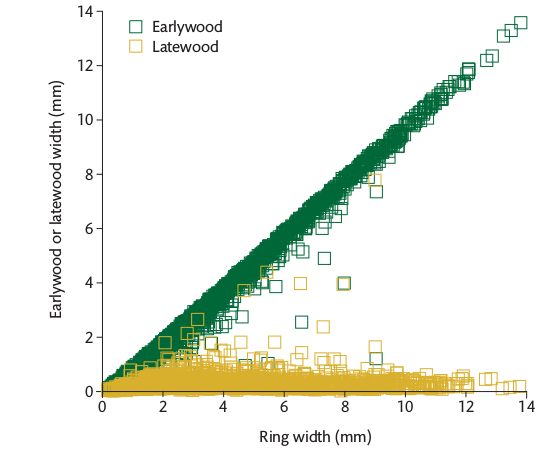
\includegraphics[width=0.65\textwidth]{wood.png}
		\caption{Largeur du bois initial et du bois final en fonction de la largeur totale du cerne chez l'épinette de Sitka \textit{Picea sitchensis}
		\citep{Moore2011}}
	    \label{fig:proportiondebois}
		
		
	\end{figure}
	

	\item \emph{Chez les semis, le stress hydrique a un effet négatif sur l'angle des microfibrilles de la paroi cellulaire. D'autre part, la sécheresse affecte négativement la conductance par la fabrication de trachéides de type \og bois final \fg jusqu'à l'arrêt total de fabrication de cellules à partir d'un certain seuil de sécheresse. Une part de la variabilité des réactions observées dans ces situations peut être attribuable aux croisements et aux clones étudiés.}\\ % AA: est-ce que tu ne travaillais pas à partir de matériel clonal?
	 
	Dans leur étude \cite{Wimmer2002} ont trouvé que la sécheresse influence l'angle des microfibrilles et \cite{Xu2012} sont allés plus loin pour comprendre cette relation. Cette dernière étude a mis évidence le fait que la température influence négativement l'angle des microfibrilles alors que les précipitations ont un impact positif. Ces études récentes offrent une perspective quant à la reconstitution du climat passé par l'étude de l'angle des microfibrilles qui, selon les travaux de \cite{Xu2012}, est plus précise que l'utilisation de la largeur des cernes. En effet, les travaux ont montré que 60\% de la variabilité de l'angle des microfibrilles est expliqué par le climat, contre 37\% de la variabilité de la largeur des cernes chez l'épinette. Les conditions de sécheresse étant rares au Québec, nous avons choisi d'induire artificiellement des changements de conditions hydriques qui devraient avoir des impacts sur l'angle des microfibrilles, les caractéristiques anatomiques du bois et la largeur des cernes. Ce choix permettra de faire un pas en avant plus rapidement dans la compréhension des effets de la sécheresse sur les propriétés du bois. Considérant le contexte actuel de changements climatiques, on peut anticiper des épisodes de sécheresse plus importants dans le futur \citep{IPCC_2015,Flato2001}. Nous nous plaçons donc dans une optique d'anticipation des effets du climat plutôt que dans celle d'une reconstitution. \\
		%AA: Ces explications sont beaucoup mieux. Par contre, il manque encore une identification des limites des connaissances actuelles. Que viendra-tu apporter de plus? On sait que la sécheresse influence les propriétés du bois, donc après tu dois identifier ta contribution à l'avancement des connaissances. Je vois trois éléments: 1. Comme la sécheresse est un phénomène inconstant en milieu naturel, il est difficile de bien l'isoler comme facteur explicatif; 2. On ne sait pas dans quelle mesure l'effet de la sécheresse sur les propriétés du bois peut varier entre les clones et les croisements; 3. l'interdépendance entre la sécheressse, la largeur de cernes et les propriétés fondamentales du bois n'a pas été modélisée explicitement. Tu ne prendras peut-être pas tous ces éléments, mais il faut faire ressortir ta contribution de manière explicite.
	
	Notre approche permettra alors de faire varier suffisamment les conditions hydriques pour mesurer une étendue complète de réactions possibles, et ce, jusqu'à l'arrêt de la croissance. Par ailleurs, l'angle des microfibrilles varie avec l'âge cambial \citep{Lindstrom1998}. Ainsi, l'utilisation d'arbres juvéniles pourrait expliquer une partie de la variabilité de l'angle des microfibrilles chez l'épinette blanche. Dans l'expérience qui sera mise en place pour cette partie, nous nous affranchirons autant que possible de cet impact potentiel en étudiant le bois opposé au bois de réaction produit par des semis dont les tiges sont inclinées, une stratégie déjà utilisée dans d'autres études \citep{Apiolaza2011}.\\  
	
	\item \emph{Une part significative de variabilité de la relation entre la proportion d'isotopes stables (\Ctreize et \Odixhuit) dans la cellulose du bois et les conditions météorologiques est associée à des différences entre les croisements.} \\
		
	La sécheresse entraîne une fermeture des stomates \citep{Farquhar1989, Farquhar1993, Nicolas2017} qui elle engendre une modification des échanges entre les feuilles et l'atmosphère et peut provoquer une augmentation de la proportion d'isotopes stables lourds (\Ctreize et \Odixhuit) \citep{McCarroll2004,Skomarkova2006,Vaganov2009,Cernusak2015}.
	
	 de la densité \citep{Drew2009, Rozas2011, Wilkinson2015}
	 et une diminution de l'angle des microfibrilles \citep{Xu2012}. %AA: Développe un peu le lien entre les isotopes et les propriétés. Donc essaie d'utiliser les proportions d'isotopes lourds comme une variable de prédiction
	 
	 
	 Également, \cite{Seftigen2011} ont remarqué que la proportion d'isotopes stables lourds (\Ctreize et \Odixhuit) croit avec l'augmentation de la température et qu'elle est corrélée négativement aux précipitations. \\
	
	La proportion de \Ctreize dans le bois est régi par la réaction de l'arbre face aux conditions climatiques, notamment la fermeture des stomates en %réponse est un anglicisme
	réaction à de fortes températures. Si l'hypothèse émise dans le premier chapitre est vérifiée et que la réaction des arbres face aux variations environnementales est héréditaire, le niveau de fermeture des stomates sera variable entre familles soumises aux mêmes stress environnementaux. Concernant la proportion de \Odixhuit dans le bois, elle est régie principalement par la quantité de précipitations et la signature isotopique de celles-ci. Si la capacité et la stratégie des arbres envers l'allocation de l'eau et du carbone à la biomasse est héréditaire \citep{Espinoza2014}, on s'attend à ce que la signature isotopique ait aussi un caractère héréditaire puisque la stratégie de transport d'eau a un impact direct sur la fermeture des stomates et la quantité d'eau absorbée. % AA: cette phrase n'est pas nécessaire puisqu'elle répète la précédente. Par conséquent, on s'attend à une part d'héritabilité entre la variabilité de la relation entre proportions de \Ctreize et \Odixhuit dans la cellulose du bois et les conditions climatiques.\\
	
	%AA: Il reste encore du travail à faire dans cette hypothèse. D'abord, il faut s'assurer du lien logique entre les trois hypothèses. La complémentarité avec la première hypothèse n'est pas évidente pour moi. Peut-être que tu peux retirer l'hypothèse sur l'hérédité dans la 2e hypothèse. Ça te permettrait ici de mieux faire valoir cette 3e hypothèse.
	
	%\cite{Drew2009} ont observé dans leur étude une variation de la densité, de l'angle des microfibrilles et de la proportion de \Ctreize suite au stress de la sécheresse. En revanche, leur étude a été faite sur une seule espèce d'arbre, \textit{Eucalyptus nitens (H.Deane \& Maiden)}, et elle a été effectuée dans des conditions d'irrigation. Il est donc important de confirmer les résultats de \cite{Drew2009} dans des conditions de stress hydrique différents et pour une autre espèce d'arbre.   
	
	 

	
\end{itemize} 


\chapter{Caractérisation des profils de densité et de la largeur des cernes afin d'identifier les familles avec le bois le plus « uniforme » face aux variations environnementales}


L'objectif de ce chapitre est d'identifier les familles d'arbres qui réagissent mieux au stress climatique, notamment le déficit hydrique.
% AA: Réagir "mieux" est un grand mot. On ne sait pas si c'est mieux pour tout. Tu pourrais dire :" identifier les familles qui montrent les réactions les moins marquées aux écarts climatiques, et qui produisent donc le bois le plus uniforme.

%AA: En passant, il faudra trouver une autre manière de travailler que dropbox dans le futur. Le problème est que tu ne verras pas la plupart de mes corrections. Souvent je dois te corriger de coquilles (pluriel, fautes d'accord, etc.). Aussi, tu disais "déterminer les familles...". On ne peut pas "déterminer" les familles. On peut déterminer quelles sont les familles qui... ou encore on peut identifier les familles. Je fais beaucoup de tels changements dans ton texte. Il faudrait que tu puisses les voir pour être en mesure d'améliorer tes textes. Si tu veux continuer de travailler avec LaTeX il te faudra travailler avec un gestionnaire de versions. Le plus facile est probablement GitHub, quoi que ce n'est pas si facile non plus..

 Nous utiliserons pour cela des données de dendrochronologie et climatiques. Les données ont été prélevées sur des arbres d'épinette blanche (\textit{Picea glauca}) plantées dans des tests de sélection génétique. 


\section*{Matériel et méthode}
\phantomsection\addcontentsline{toc}{section}{Matériel et méthode}

\subsection*{Site et matériel}

Le matériel utilisé dans cette étude est issus de sélection génétique pour une série de tests % AA: que veux-tu dire par "plus importante?
%AS Modifié
 en fonction des provenances ou de la région géographique \citep{Beaulieu1996}. Ces tests génétiques ont été mis en place à partir de semis d'épinette blanche (\textit{Picea glauca} (Moench) Voss) cultivés en pépinière et plantés à l'âge de 2 ans. L'un de ces sites est situé près de Saint-Casimir, au Québec, dans la zone écologique de l'érablière à tilleul, et l'autre près de Cabano (Asselin), au Québec, dans le domaine de la sapinière à bouleau jaune. Cette série d'essais a été établie en 1999 par le Service canadien des forêts et elle représente l'une des trois parties essentielles du programme d'amélioration de l'épinette blanche au Québec. Les essais ont été réalisés par blocs, dans lesquels chaque famille était représentée par cinq arbres dans une rangée-parcelle. L'espacement entre les arbres était de 2 m en disposition orthogonale. Les échantillons utilisés dans ce travail ont été récoltés sur 93 familles, 2500 individus, 1250 arbres / site. Les mesures de densité, de la largeur des cernes et de l'angle des microfibrilles ont été prises à hauteur de poitrine (1,3 m du sol) dans la tige de chaque arbre échantillonné. Les carottes utilisées pour les différentes mesures ont été prélevées en 2014-2015.  \\ 

Pour vérifier la précision des datations et déterminer les cernes manquants,  nous avons utilisé COFECHA qui est un programme de dendrochronologie qui sert pour la datation croisée et le contrôle de la qualité des mesures sur les cernes annuels \citep{HOLMES1983}. Ainsi, comme la séparation des cernes annuel avait été effectuée par un algorithme, nous avons éliminé les échantillons dont la datation n'est pas correcte. 

 %mettre le type de sol

\subsection*{Détermination de la densité}
La densité du bois est mesurée sur deux rayons sur chaque disque pris à partir d'une hauteur déterminée (c'est-à-dire 1,3 m) sur une face commune (face Nord). Les échantillons de carottes sont ensuite extraits au Soxhlet pendant une nuit avec de l'acétone, coupés avec précision à 1,68 mm d'épaisseur avec une scie pneumatique à deux lames, et laissés à 7\% d'humidité avant l'analyse de densité. 
Tous les échantillons sont ensuite scannés de la moelle à l'écorce par densitométrie à rayons X (Quintek Measurement Systems, TN) à une résolution de 0,0254 mm, et les données sont rapportées en tant que densité relative sur une base de poids sec. % AA: Il te faudrait aussi donner la teneur en humidité pour le volume. Normalement on utilise la densité basale qui est la masse anhydre sur le volume saturé.

\subsection*{Données climatiques}
Les données climatiques (la température et les précipitations) ont été générées par le logiciel BioSim. BioSIM est un logiciel conçu pour aider à l'application de modèles de simulation axés sur la température et les précipitations \citep{Regniere2014}. Les intrants qui ont été fournis à BioSIM pour qu'il puisse faire les simulations relatives à la température et aux précipitations sont les données de latitude, de longitude et l'élévation de chaque site d'étude. Ainsi, BioSim utilise les données des stations météo les plus proches autour de chaque site d'étude pour générer les données climatiques du site. 
Les stations météorologiques sont utilisées dans le calcul avec des pourcentages pondérés qui sont proportionnels à la distance de la station par rapport à la localisation du site.\\ 

Le lien entre les données météorologiques et la largeur des cernes sera fait à l'aide du logiciel DENDOCLIM2002 complété par des modèles statistiques. Dendoclim permet de calibrer la chronologie des cernes par rapport aux données climatiques en utilisant des fonctions de corrélation et de réaction. Il permet de mettre en évidence la corrélation entre cernes et climat \citep{Biondi2004}. 

\subsection*{Analyses statistiques}
Plusieurs données ont été récoltées sur les arbres des deux sites d'étude. Dans le cas de ce chapitre, nous utiliserons la densité du bois et la largeur des cernes annuels. Concernant les paramètres environnementaux, nous utiliserons principalement les températures moyennes mensuelles et les précipitations moyennes mensuelles. Dans notre analyse, nous mettrons en relation la densité du bois et la largeur des cernes avec les facteurs environnementaux. \\

%AA: Pour le choix de la résulution mensuelle, tu peux t'appuyer sur cet article:
%
%@article{franceschini2017effect,
%	title={Effect of thinning on the relationship between mean ring density and climate in black spruce (Picea mariana (Mill.) BSP)},
%	author={Franceschini, Tony and Gauthray-Guy{\'e}net, Vincent and Schneider, Robert and Ruel, Jean-Claude and Pothier, David and Achim, Alexis},
%	journal={Forestry: An International Journal of Forest Research},
%	pages={1--16},
%	year={2017}
%}

% Par contre, il faut voir qu'un mois est une limite arbitraire, et qu'en plus, les mois d'une même année sont autocorrélés. Il faudra donc raffiner les analyses afin d'éviter ces problèmes.

Nous utiliserons des modèles linéaires mixtes pour le traitement de données notamment le contrôle génétique.
% AA: "le traitement de données notamment le contrôle génétique." ne veut pas dire grand-chose. Il faut clarifier cette affirmation

 Les données contiennent des variables fixes et des variables aléatoires ce qui explique le choix d'utiliser des modèles mixtes, car les tests d'ANOVA classiques ne permettent pas l'utilisation de plusieurs facteurs aléatoires.
 
Les variables à effets aléatoires seront les facteurs site, individu, année (largeur des cernes) et densité.

% Variable dépendante: densité
% Effets fixes: prédcipitations, indices de sécheresse, croisement 
% Effet aléatoire: site (pas idéal parce qu'on n'en a que 2, mais ça respectera la structure de la variance), bloc, arbre

% AA: Année n'est pas la même chose que largeur de cerne. Aussi, c'est le niveau le plus fin de la structure de la variance dans ton analyses. Donc l'année ira dans l'erreur résiduelle du modèle. La largeur du cerne ne sera pas un effet alétaoire non plus, mais peut-être un effet fixe. La densité n'est ni un effet fixe, ni un effet aléatoire. C'est la variable que tu souhaites prédire (variable dépendante)

 Les variables à effet fixes seront la famille et le climat. Nous nous servirons du logiciel R \citep{R2018} et plus spécifiquement du package NLME \citep{NLME2018} pour la construction de nos modèles linéaires mixtes. Le package ASReml sera utilisé pour calculer l'héritabilité et les corrélations génétiques. Deux modèles seront construits, un modèle pour le bois initial avec les données environnementales du printemps et un deuxième pour le bois final avec les données climatiques de l'été.
 
 %AA : En lien avec un commentaire précédent : tu dois démêler ce qui sera présenté comme analyse des effets des familles. Ton début de chapitre dit que tu souhaites identifier les familles ayant une réaction différente au climat. Ici tu parles de calculer l'héritabilité. Ce n'est pas la même chose. Il faudrait que cet aspect devienne plus clair.

\section*{Résultats attendus}
\phantomsection\addcontentsline{toc}{section}{Résultats attendus}

Nous nous attendons à avoir dans nos résultats des familles ayant des propriétés (largeur des cernes et densité) plus "uniformes", donc moins sensibles à la variabilité de la  température et des précipitations entre les différentes années.\\ 

Les arbres où les familles qui ont des largeurs de cernes et ou une densité peu sensibles aux fluctuations des conditions métrologiques seront considérés comme résistants aux variations climatiques. Ces arbres auront donc un bois de densité plus constante que les autres d'une année à l'autre, sans forte augmentation de la proportions de bois initial pour les années avec conditions climatiques favorables et avec une décroissance moins marquée de la largeur des cernes les années sèches durant lesquelles les conditions climatiques sont moins favorables à la croissance. Dans le contexte des changements climatiques où l'on s'attend à de des sécheresses plus fréquentes et sévères \citep{IPCC_2015}, nous croyons que ces familles auront des caractéristiques intéressantes pour le reboisement. Il est logique d'assumer que les arbres avec peu de variations seront résilients au écarts climatiques, mais cette affirmation ne sera pas vérifiée dans le cadre de cette thèse. L'identification des familles produisant du bois de densité uniforme sera donc effectuée dans une optique de sélection d'une propriété avantageuse pour la transformation des produits \citep{Hernandez2001}. \\ %AA: Remarque l'ajustement que j'ai fait aux deux dernières phrases. Je pense qu'il sera important de conserver cette idée et de bien la présenter. Comme ça tu ne t'exposeras pas à la critique par rapport à la résilience (qu'on ne mesure pas)

Les familles d'arbres les plus sensibles auront quant à elles une variation importante de la largeur et de la densité des cernes annuels en lien avec les fluctuations des conditions environnementales. Il faut rappeler que la largeur des cernes d'une année à l'autre est influencée principalement par le bois initial \citep{Moore2011}. 
Ces familles plus sensibles auront un bois avec des cernes plus larges les années où la météo est favorable et une proportion de bois initial important. Par conséquent, elles auront une densité faible et inversement pour les années avec conditions climatiques peu favorables.\\

%AA: On a complètement perdu le lien avec ton hypothèse. Remaque que c'est peut-être l'hypothèse qui est à changer... On doit en parler de vive-voix

\section*{Conclusion}
\phantomsection\addcontentsline{toc}{section}{Conclusion}

L'identification des familles d'arbres qui ont des cernes "uniformes" malgré les variations environnementales, permettra de faire une meilleure sélection pour le reboisement au Québec et plus largement au Canada. L'amélioration génétique des forêts permettra ainsi de prendre en compte la productivité et la qualité du bois dans un contexte de climat changeant.\\

Cette partie du projet permettra de faire une sélection des familles qui serviront au reboisement. Par contre, cela reste limité si nous prenons en compte les prédictions climatiques futures dans la mesure où ces arbres n'ont pas connu des sécheresses intenses comme prévu dans les prédictions. Dans le chapitre 2 de ce projet, nous prendrons en compte l'intensité et la durée de la sécheresse par la mise en place d'une expérimentation en serre dans laquelle nous prendrons en compte de nouveaux facteurs notamment l'angle des microfibrilles en plus de ceux utilisés dans le premier chapitre. Le chapitre 2 permettra l'identification des arbres les plus résistants à la sécheresse intense ainsi que l'héritabilité de ces facteurs.  



\chapter{Modélisation de l'impact d'une sécheresse plus ou moins intense sur l'angle des microfibrilles, la densité et l'héritabilité de la réaction du bois face à ce stress}


L'objectif de ce chapitre est 1) de mieux comprendre les effets de différents niveaux de sécheresse sur les propriétés du bois et 2) de déterminer quelles familles d'arbres produisent le bois aux caractéristiques les plus avantageuses en situation de stress hydrique. Les propriétés prises en compte dans ce chapitre seront principalement l'angle des microfibrilles et la masse volumique du bois. Une expérience botanique sera mise en place pour une meilleure maîtrise de l'intensité et de la fréquence de la sécheresse sur une période relativement longue.   

%AA: Dans ton hypothèse tu avais aussi la conductivité du xylème. Il faudrait l'ajouter ici. Voir aussi les méthodes ci-bas qui devront être ajustées.

\section*{Matériel et méthode}
\phantomsection\addcontentsline{toc}{section}{Matériel et méthode}

\subsection*{Site et matériel}

Le matériel utilisé dans cette étude sera issu de sélection génétique pour une série de tests plus importante en fonction des provenances ou de la région géographique pour le reboisement de l'épinette blanche au Québec \citep{Beaulieu1996}. Dans ce volet de notre étude, une expérimentation sera mise en place en serre avec environ 420 plants issu d'embryogenèse provenant de 11 croisements dirigés plein-frères avec une hauteur d'environ 42 cm (Voir figure~\ref{plant}). Dans la serre les conditions environnementales seront contrôlées. L'expérience sera composée de trois traitements, un témoin (conditions environnementales optimales),
%AA: note qu'on ne dit pas "contrôle" en français, mais témoin
un avec faible stress hydrique imposé et le dernier avec un stress hydrique plus intense. Les principaux facteurs environnementaux qui seront contrôlés sont la température de l'air, l'humidité du sol, la quantité d'eau apportée (précipitations). Une charge sera posée sur les tiges des semis afin de les obliger à faire du bois de réaction d'un côté et du bois normal de l'autre. 
Le bois normal sera utilisé pour les analyses, ainsi nous nous affranchirons des effets du bois de flexion produit dans les premières années de la vie d'un arbre. %AA: voici une meilleure manière de présenter le bois de flexion. Cite l'étude suivante

%@article{telewski1989structure,
%	title={Structure and function of flexure wood in Abies fraseri},
%	author={Telewski, FW},
%	journal={Tree Physiology},
%	volume={5},
%	number={1},
%	pages={113--121},
%	year={1989},
%	publisher={Heron Publishing}
%}

 L'expérience sera réalisée sur une durée de deux ans. Après la première année, une partie des semis sera coupée et analysée.\\


\begin{figure}
	
	\centering
	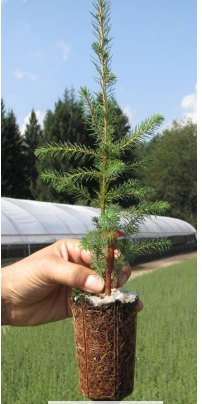
\includegraphics[width=0.35\textwidth]{plant_epinette.png}
	\caption{Plant d'épinette blanche. (Par Julie Gravel Grenier, Pépinière de Saint-Modeste)}
	\label{plant}	
	
\end{figure}

%AA: Il te manque une description de ton plan d'expérience. Combien de familles? Combien de répétitions? Plan entièrement aléatoire ou en blocs?


\subsection*{Détermination de l'angle des microfibrilles}
L'angle des microfibrilles sera déterminé à l'aide de diffractomètre à rayon-X SilviScan-3. Les échantillons d'arbres seront scannés de la moelle à l'écorce et la moyenne de l'angle des microfibrilles calculée sur un intervalle de 3 mm. 
Les informations données par les profils de diffraction nous permettront d'avoir l'orientation moyenne des microfibrilles dans la couche S2 de la paroi cellulaire secondaire \citep{Evans1999}. %AA Idéalement il faudrait donner la résolution de la mesure. Je crois qu'elle sera de 2 mm.

\subsection*{Détermination de la densité}
La densité du bois sera mesurée à l'aide d'un densitomètre à rayon-X. 
Cette mesure permettra d'établir un profil de densité pour les deux cernes annuels produits par l'arbre.

 %AA: Il faudrait faire un montage complexe pour y arriver. Ça ne sera pas si simple que ça. Je te propose d'utiliser plutôt des coupes analtomiques comme Yann l'a fait. En plus, pour mesurer la conductivité tu auras besoin de ces coupes anatomiques.


\subsection*{Analyses statistiques et héritabilité}
Les données récoltées après l'expérience seront traitées statistiquement pour déterminer la significativité des variations de la densité, de l'angle des microfibrilles et de %l'héritabilité. AA: l'héritabilité est une mesure que tu ne sembles pas maitriser. Tu est mieux de ne pas en parler pour le moment. Il te manque la conductivité dans cette énumération.

 Les paramètres environnementaux seront principalement ceux contrôlés lors de l'expérience notamment, les températures moyennes mensuelles et le niveau de sécheresse (quantité d'eau apportée).
%AA: Non, tu ne travailleras pas avec les températures, mais uniquement avec les traitements prévus dans ton expérience

Dans cette analyse, nous mettrons en relation d'une part, la densité du bois et l'angle des microfibrilles avec les facteurs environnementaux et d'autre part, l'héritabilité de la réaction des semis face à la sécheresse. \\ %AA encore une fois, je pense qu'il ne faut pas parler d'héritabilité pour le moment. Tu est mieux de prévoir 2 types d'analyses: 1) Mesurer les effets des traitement de sécheresse sur chacune des propriétés mesurées (densité, AMF, conductivité) et voir dans quelle mesure une part significative de la variance est reliée à la famille (ou au clone, le cas échéant); 2) analyser les corrélations entre les changements de croissance induits par la sécheresse et les changements de densité, AMF et conductivité.

Nous utiliserons des modèles linéaires mixtes pour le traitement de données comme dans le premier chapitre de notre de nos travaux. Les variables à effets aléatoires sont les individus, la densité et l'angle des microfibrilles. %AA: Attention: tu ne comprends clairement pas ce que sont les effets fixes et aléatoires. On doit en parler ensemble. La densité et l'AMF ne peut pas être un effet aléatoire dans ces analyses. Ce sont tes variables dépendantes

%Variables dépendantes: angle des microfibrilles, conductivité
% Effets fixes: traitements (3 niveaux)
% Effets aléatoires: bloc?

Les variables à effet fixes sont la famille et le niveau de sécheresse. Le logiciel R sera utilisé pour la construction de nos modèles linéaires mixtes. 

\section*{Résultats attendus}
\phantomsection\addcontentsline{toc}{section}{Résultats attendus}

Dans les résultats de cette expérience, on s'attend à avoir une répartition des arbres par famille en fonction de la réaction face à la sécheresse. 
Certaines familles seront moins sensibles que à d'autres à la variation du niveau de sécheresse. Les familles peu sensibles auront une densité et un angle des microfibrilles "uniforme" face aux variations des conditions environnementales.\\ %AA l'uniformité ne peut pas être ce qu'on mesure ici sur 2 ans. Il faut plutôt se rapporter aux différences entre les témoins et les arbres traités. On peut aussi faire un lien entre la conductivité et les autres propriétés. La section qui suit manque d'étoffe et elle doit être réécrite. Tu dois mieux utiliser le lien avec tes hypothèses et la littérature sur le sujet. 

Les arbres qui auront une densité et un angle des microfibrilles peu sensibles aux fluctuations des conditions environnementales seront considérés comme résistants. Ces arbres auront donc une densité du bois constante malgré la variation de la sécheresse. Ces familles seront identifiées et sélectionnées dans le cadre du reboisement au Québec. \\

On s'attend à avoir une augmentation de la densité du bois des familles sensibles pour une sécheresse à intensité faible ou moyenne et une chute de celle-ci pour une sécheresse à forte intensité. De plus, ces familles auront un angle des microfibrilles qui décroît avec l'intensité de la sécheresse. 


\section*{Conclusion}
\phantomsection\addcontentsline{toc}{section}{Conclusion}

Cette expérience permettra de mieux comprendre l'impact d'une sécheresse intense et constante sur les propriétés du bois formé. Ainsi, nous pourrons identifier les familles les plus résistantes à la sécheresse. % AA: je n'aime pas cette affirmation parce que tu ne mesureras pas la résistance à la sécheresse. tu pourrais dire: "Ainsi, nous pourrons mieux comprendre comment les mécanismes d'adaptation aux conditions de sécheresse peuvent varier entre les familles. J'aurais aimé que tu nous parle de trade-offs en lien avec la littérature. Par exemple, pour rendre le bois plus résistant aux embolies, il est possible de changer l'anatomie des cellules en produisant une paroi plus épaisse, et donc un bois plus dense. Par contre, il est possible que le coût en biomasse soit élevé, contrairement à une autre adaptation qui consisterait à produire une paroi avec un angle des microfibrilles plus faible. Donc il est possible que ces deux adaptations ne soient pas toujours associées. Tu vois le genre d'idées? J'aurais aimé que tu fouilles un peu plus pour nous proposer quelque chose de plus significatif comme analyse. Il se fait tard, mais tu dois au minimum nous présenter des idées plus en lien avec ton hypothèse de départ.

Quoique les familles d'arbres les plus sensibles aient un angle des microfibrilles faible et donc plus rigide, les familles les moins sensibles à ce stress seront sélectionnées pour le reboisement car l'angle des microfibrilles serait le seul facteur avantageux parmi les propriétés mécaniques du bois en cas de forte sécheresse. Les résultats de l'étude pourront servir pour l'amélioration génétique qui pourra faire des croisement entre familles les plus résistantes pour la densité et celles qui ont une meilleure rigidité.\\

Cette seconde partie du projet servira à faire une sélection des familles qui servirons au reboisement et aussi à l'amélioration génétique. Il a été mis en évidence dans des études antérieures qu'il existe une relation entre la proportion d'isotopes stables (\Ctreize et \Odixhuit) et les conditions environnementales avec peu de connaissances sur l'héritabilité de la signature isotopique.  Par conséquent, dans le chapitre 3 de ce projet, nous prendrons en compte ce nouveau facteurs en plus de ceux étudiés dans les 2 chapitres précédents. Ce chapitre permettra l'identification des arbres les plus résistante à la sécheresse et la caractérisation du stress climatique au niveau du bois par la signature isotopique ainsi que l'héritabilité de ce dernier facteur.


\chapter{Estimation de l'héritabilité de la proportion d'isotopes stables (\Ctreize et \Odixhuit) face aux variations climatiques chez \textit{Picea glauca}}

%AA : ajuster le titre et les hypothèses pour ne plus parler d'héritabilité (pas pour pour le moment du moins). On peut garder la même ligne tout au long du proposé, soit celle d'identifier des différences entre les familles. Les analyses isotopiques coûtent trop cher pour qu'on puisse avoir suffisamment d'échantillons pour qu'on puisse mesurer l'héritabilité.

Les objectifs de ce chapitre sont 1) de quantifier les effets des conditions météorologiques su la proportion d'isotopes stables lourds dans la cellulose du bois et 2) de déterminer dans quelle mesure cette proportion peut varier entre les familles analysées. 

\section*{Matériel et méthode}
\phantomsection\addcontentsline{toc}{section}{Matériel et méthode}

\subsection*{Site et matériel}
%AA Recopier les petites corrections que j'ai effectuées dans le texte semblable du chapitre 1.
Le matériel utilisé dans ce chapitre est issus de sélection génétique pour une série de test plus importante en fonction des provenances ou de la région géographique \citep{Beaulieu1996}. Ces tests génétiques ont été mis en place à partir de semis d'épinette blanche (\textit{Picea glauca} (Moench) Voss) cultivés en pépinière âgés de 2 ans. L'un de ces sites est situé près de Saint-Casimir, au Québec, dans la zone écologique érable-tilleul, et l'autre près de Cabano, au Québec, dans la zone de sapin baumier-jaune. Cette série d'essais a été établie en 1999 par le Service canadien des forêts et il représente l'une des trois parties essentielles du programme d'amélioration de l'épinette blanche au Québec. Les essais ont été faits par blocs, où chaque famille était représentée par cinq arbres dans une rangée-parcelle par bloc. L'espacement entre les arbres était de 2 m dans toutes les directions.  Les données utilisé dans ce travail ont été récolté sur 93 familles, 2500 individus, 1250 arbres / site. Les mesures de densité, de la largeur des cernes et de l'angle des microfibrilles ont été prises au niveau du diamètre à hauteur de poitrine (DHP, environ 1,3m du sol) pour chaque arbre échantillonné. Les carottes utilisé pour les différentes mesures ont été prélevés en 2015.  \\

\subsection*{Détermination de la densité}
%AA: même chose ici. Reprendre les corrections. Remarque que la répétition n'est pas nécessaire. Tu peux aussi référer au chapitre 1, tout simplement.
La densité du bois est mesurée sur deux rayons sur chaque disque pris à partir d'une hauteur déterminée (c'est-à-dire 1,3 m ou DHP) sur une face commune (face Nord). Les échantillons de carottes sont ensuite extraits au Soxhlet pendant une nuit avec de l'acétone, coupés avec précision à 1,68 mm d'épaisseur avec une scie pneumatique à deux lames, et laisser à 7\% d'humidité avant l'analyse de densité. Tous les échantillons sont ensuite scannés de la moelle à l'écorce par densitométrie aux rayons X (Quintek Measurement Systems, TN) à une résolution de 0,0254 mm, et les données sont rapportées en tant que densité relative sur une base de poids sec. 

\subsection*{Détermination de l'angle des microfibrilles}
L'angle des microfibrilles sera déterminé par diffraction des rayons X en déterminant l'arc de diffraction 002 (T-values) en utilisant une unité de diffraction des rayons X Bruker D8 Discover équipée d'un détecteur (GADDS) sur la face radiale des anneaux de croissance individuels. La diffraction grand angle sera utilisée dans le mode de transmission, et les mesures sont effectuées avec CuK$\alpha$1 radiation ($\lambda$ = 1.54A), la source de rayons X sera ajustée avec un collimateur de 0,5 mm et le photon diffusé recueilli par le détecteur GADDS. La source de rayons X et le détecteur seront réglés sur theta = 0 °. La valeur T moyenne (la moitié de la distance entre les points d'intersection des tangentes aux courbes d'intensité et l'axe des abscisses) des deux pics d'arc de diffraction 002 sera utilisée comme valeurs T pour générer la courbe des calculs d'angle de microfibrille. Des sections de bois des cernes ont été préalablement sélectionnées sur la base de la distribution de la valeur T de la diffraction des rayons X et de la symétrie du profil, et analysées par microscopie photonique composée comme décrit par \cite{Wang2001} à un grossissement de 400x utilisant la microscopie différentielle à contraste interférentiel pour générer des courbes de régression pour les espèces, y compris l'épinette. Les intervalles de confiance ($\lambda$ = 0,05) seront calculés, avant de numériser une population d'échantillons. Par conséquent, l'angle de microfibrilles de tous les échantillons de bois subséquents a ensuite été estimé en mesurant l'intensité du pic 002 pour la portion de bois de chaque échantillon à un âge commun de la moelle, par exemple.

%AA: tu n'as rien sur les mesures isotopiques! Tu peux dire qu'on va couper des séries de tranches d'une épaisseur de 100 microns dans quatre directions cardinales principales. Ces tranches seront prélevées en séquence au microtome du bois initial au bois final. Le bois des 4 directions sera mélangé, la cellulose sera extraite et sera broyée. Les échantillons seront par la suite envoyés au "Delta Lab" de la Commission géologique du Canada où les proportions de 13C et 18O seront mesurées.

%AA: je te laisse terminer cette section.


\subsection*{Analyses statistiques}
Les données seront traitées statistiquement pour déterminer l'héritabilité de la composition isotopique en carbone et en oxygène. Dans cette analyse, nous mettrons en relation d'une part, la signature isotopique du bois avec les facteurs environnementaux et d'autre part, l'héritabilité de la réaction en isotopes stables en fonction des variations climatiques. \\

Comme précédemment,  nous utiliserons des modèles linéaires mixtes pour le traitement de données. Les variables à effets aléatoires sont les individus, la proportion d'isotopes stables lourds. Les variables à effet fixes sont la famille et les facteurs environnementaux. Le logiciel R sera utilisé pour la construction de nos différents modèles. 

\section*{Résultats attendus}
\phantomsection\addcontentsline{toc}{section}{Résultats attendus}

Dans ce chapitre, on s'attend d'une part, à avoir une relation entre la composition isotopique du bois et les autres propriétés du bois (densité, largeur des cernes et angle des microfibrilles) et d'autre part, une relation entre la signature isotopique et les variations climatiques comme d'autres études l'ont déjà montré. Ensuite, nous nous attendons à voir une composition isotopique similaire chez les individus issus de la même famille. Si l'héritabilité est vérifié, les familles les moins sensibles (densité et angle des microfibrilles relativement uniforme) auront une signature isotopique plus ou moins constante d'une année à l'autre. 

\section*{Conclusion}
\phantomsection\addcontentsline{toc}{section}{Conclusion}

Les résultats de ce chapitre de notre étude permettront à la fois une déduction des variations climatiques et une caractérisation de l'héritabilité de la réaction des arbres face aux stress environnementaux par la proportion d'isotopes stables (\Ctreize et \Odixhuit) dans le bois. Les analyses isotopiques provienne de la molécule, ce qui augmente leur précision comparé à d'autres analyses. Ainsi, si on obtient les résultats escomptés, les analyses isotopiques permettrons de pouvoir décrire de manière plus fine les conditions environnementales de la production du bois et l'héritabilité peut réduire le nombre d'échantillons dans le cas des forêts constituées de population issus de sélection génétique. 

\clearpage % passer à la page suivante

\chapter*{Conclusions et perspectives}
\phantomsection\addcontentsline{toc}{chapter}{Conclusions et perspectives}

L'amélioration génétique a longtemps servi à l'augmentation de la production du bois sans prendre en compte de la qualité de celui-ci. La qualité du bois est de plus en plus prise en compte. Le bois est davantage utilisé pour substituer au  béton ou à l'acier dans la société d'aujourd'hui, il est d'autant plus important qu'il soit de qualité. La possibilité de remplacer certains matériaux notamment le béton et l'acier par le bois est positif pour freiner les changements climatiques du fait que le bois stock le carbone. La prédiction des effets potentiels des changements climatiques sur la production et la qualité du bois permet d'anticiper ceux-ci et d'adapter le choix des semis utiliser pour le reboisement des forêts. \\

Cette thèse donnera certains outils pour anticiper les effets potentiels des variations environnementales sur la qualité du bois. La caractérisation de l'impact des conditions météorologiques sur les propriétés (densité, largeur des annaux de croissance annuelle, l'angle des microfibrilles et la signature isotopique) du bois permet une sélection des familles les mieux adaptées aux variations climatiques. L'amélioration génétique sera alors un outil efficace pour une production optimale de bois de bonne qualité. La densité chute à partir d'un certain niveau de stress dû à la sécheresse, contrairement à l'angle des microfibrilles qui semblent continués à croître. Par contre, des études récentes ont trouvés que d'autres facteurs anatomiques notamment les auxines influencent l'angle des microfibrilles \citep{Korbei2011,Chan2012}. Certaines familles d'arbres peuvent être peu sensibles au stress hydrique en ayant une anatomie qui favorise la formation de bois avec un faible angle des microfibrilles. Ces familles auront alors un potentiel intéressant pour le reboisement du fait qu'elles sont résistante aux variations climatiques quoi qu'elles aient un bois avec une forte rigidité. \\
Si une corrélation est observée entre densité, largeur de cerne, angle de microfibrille, sécheresse et la proportion d'isotopes stables lourds (\Ctreize et \Odixhuit) alors la signature isotopique de par sa précision pourra être utilisée afin d'avoir des informations à la fois sur les conditions climatiques et sur les les différentes propriétés du bois. L'interdisciplinarité de cette thèse lui permettra de contribuer à l'avancée des connaissances fondamentales de la science et aussi l'application des découvertes scientifiques par la sélection des familles pour le reboisement des forêts futures. 

\clearpage

\begin{landscape}
	
\begin{figure}
	\includegraphics[width=1.1\columnwidth]{Calendrier.pdf}
	\caption{Calendrier prévisionnel de la thèse}
	\label{fig:calendrier}
	\end{figure}

\end{landscape}
 
\bibliography{bibliographie}
\bibliographystyle{apalike}
\end{document}